\section{序列二次规划}
\label{sec:opt-con-sqp}

惩罚法与乘子法把约束问题变成一串无约束问题，每个内层问题本身还要迭代很多步。对光滑的非线性约束问题，还可以像第~\ref{chap:opt-smooth}章的牛顿法那样，直接在当前点建立一个局部模型，一步解出模型的最优步。约束问题的局部模型是一个二次规划：目标用二阶信息近似，约束用一阶信息线性化。本节先说明这个子问题怎样构造、求解时会遇到什么障碍；再说明模型给出的步怎样放回原问题检验，以及在什么条件下这一方法收敛得很快。它与第~\ref{sec:opt-con-interior-point}节沿可行域内部路径前进的内点法是两种不同的思路。

\subsection{局部二次子问题}
\label{sec:opt-con-sqp-subproblem}

\paragraph{子问题的构造}
设当前迭代为$\bm x^{(t)}$，乘子估计为$(\bm\lambda^{(t)},\bm\nu^{(t)})$，以步向量$\bm p$为未知量。约束线性化为$h_j(\bm x^{(t)})+\langle\nabla h_j(\bm x^{(t)}),\bm p\rangle=0$与$g_i(\bm x^{(t)})+\langle\nabla g_i(\bm x^{(t)}),\bm p\rangle\leq0$；目标取一阶项加上Lagrange函数的曲率：
\begin{equation}
\label{eq:opt-con-sqp-subproblem}
  \min_{\bm p}\ \langle\nabla f(\bm x^{(t)}),\bm p\rangle+\frac12\bm p^\top\bm H_t\bm p
  \quad\text{s.t.}\quad
  \bm h+\bm J_h\bm p=\bm0,\quad\bm g+\bm J_g\bm p\leq\bm0,
\end{equation}
其中$\bm h,\bm g$与Jacobian $\bm J_h,\bm J_g$都在$\bm x^{(t)}$处取值，$\bm H_t=\nabla^2_{\bm x\bm x}\mathcal L(\bm x^{(t)},\bm\lambda^{(t)},\bm\nu^{(t)})$或它的拟牛顿近似。这是第~\ref{sec:opt-con-qp}小节定义的二次规划。逐项看：目标梯度决定一阶下降方向；约束残差$\bm h,\bm g$决定线性化约束要求步子修正多少违约；Jacobian决定约束怎样随步子变化；曲率用的是$\nabla^2\mathcal L$而不是$\nabla^2f$，因为沿弯曲的约束面移动时，约束的曲率也会改变目标值，乘子把这部分曲率加了进来。子问题的乘子就是下一轮的乘子估计。反复求解这样的子问题称为\term{序列二次规划}（sequential quadratic programming，SQP）。

\paragraph{等式约束：KKT线性系统}
只有等式约束时，子问题的KKT条件是线性方程组
\begin{equation}
\label{eq:opt-con-sqp-kkt}
  \begin{bmatrix}\bm H_t&\bm J_h^\top\\\bm J_h&\bm0\end{bmatrix}
  \begin{bmatrix}\bm p\\\bm\nu^{(t+1)}\end{bmatrix}
  =-\begin{bmatrix}\nabla f(\bm x^{(t)})\\\bm h(\bm x^{(t)})\end{bmatrix}.
\end{equation}
它恰好是对原问题的KKT方程组$\nabla f+\bm J_h^\top\bm\nu=\bm0$、$\bm h=\bm0$作一步牛顿线性化的结果（在$\bm H_t$取精确Hessian时），所以SQP可以看作对KKT条件使用牛顿法。

考虑$\min x_1+x_2$、约束$x_1^2+x_2^2=2$。最优点$\bm x^\star=(-1,-1)^\top$，由$(1,1)^\top+\nu(2x_1,2x_2)^\top=\bm0$得$\nu^\star=1/2$。$\nabla^2_{\bm x\bm x}\mathcal L=2\nu\bm I$。从$\bm x^{(0)}=(0.2,-1.6)^\top$、$\nu^{(0)}=1$出发：$h=0.04+2.56-2=0.6$，$\bm J_h=(0.4,-3.2)$，$\bm H_0=2\bm I$。方程组第一行给出$\bm p=-\frac12\bigl((1,1)^\top+\nu^{(1)}(0.4,-3.2)^\top\bigr)$，代入第二行$\bm J_h\bm p=-0.6$得$-\frac12(-2.8+10.4\nu^{(1)})=-0.6$，于是$\nu^{(1)}=4/10.4\approx0.385$，$\bm p\approx(-0.577,0.115)^\top$，$\bm x^{(1)}\approx(-0.377,-1.485)^\top$。图~\ref{fig:opt-con-sqp}画出后续迭代：第一个子问题的线性化约束（黄色虚线）是圆在$\bm x^{(0)}$附近的切线方向平移，新点落在这条直线上而不在圆上；之后迭代很快靠近最优点，约束值依次为$0.6,0.346,0.897,0.076,8\times10^{-4},\dots$，前几步并不单调，进入最优点附近后每步误差大致平方。

\begin{figure}[!htbp]
  \centering
  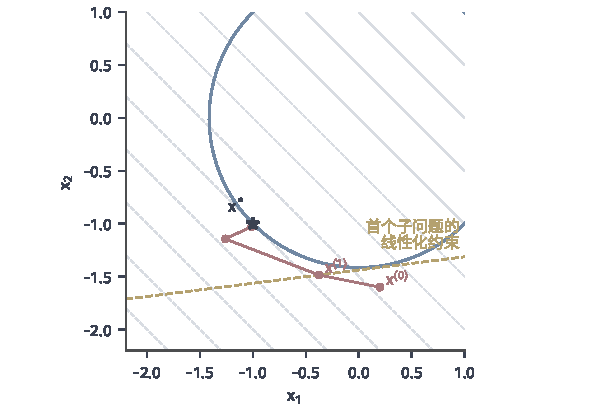
\includegraphics[width=100mm]{figures/03-optimization-evolution-and-signals/01-optimization/matplotlib/c5-sqp/figure.pdf}
  \caption{$\min x_1+x_2$、$x_1^2+x_2^2=2$上的SQP迭代（精确Lagrange Hessian，全步长）。蓝色圆为可行域，灰色虚线为目标等值线，黄色虚线为第一个子问题的线性化约束。红色折线从$\bm x^{(0)}=(0.2,-1.6)^\top$出发，约5步到达五角星$\bm x^\star=(-1,-1)^\top$；中间迭代点不在圆上。}
  \label{fig:opt-con-sqp}
\end{figure}

\paragraph{不等式与活动集}
含不等式时，子问题~\eqref{eq:opt-con-sqp-subproblem}要用二次规划方法求解（如第~\ref{sec:opt-con-qp}小节的活动集思路），它在线性化约束中选出当前需要以等号处理的那些。在满足严格互补等条件的解附近，子问题选出的活动集与原问题最优点的活动集相同，此后SQP就像在固定活动集上的等式约束牛顿法；远离解时，活动集可能在相邻迭代之间反复变化。

\paragraph{子问题可能不可用}
子问题不是每次都能直接给出一个好步。第一种障碍是曲率：若$\bm H_t$在线性化约束的零空间上不正定，二次规划可能无下界或只有鞍点。$\nabla^2\mathcal L$在远离解处完全可能不定，例如上例若乘子估计为负，$2\nu\bm I$就是负定的。常用的修正是给$\bm H_t$加上$\delta\bm I$直到零空间上正定，或者用保持正定的拟牛顿更新（如阻尼BFGS，第~\ref{chap:opt-smooth}章）代替精确Hessian。第二种障碍是线性化约束本身无解。仍看上例，若在原点处线性化，$\bm J_h=(0,0)$、$h=-2$，线性化约束成为$0=2$，子问题不可行，而原问题是可行的。这时需要可行性恢复：暂时改为最小化线性化约束的违约（例如引入松弛变量的弹性子问题），先回到线性化相容的区域。两种障碍都意味着不能默认每轮都得到可以直接采用的下降步。

\subsection{模型步的接受与收敛}
\label{sec:opt-con-sqp-acceptance}

\paragraph{用评价函数检验模型步}
子问题的解只在模型里最优。把$\bm x^{(t)}+\bm p$放回原问题时，目标可能变差、约束违约也可能变大（上例第二步约束值就从$0.346$升到$0.897$）。目标与约束可能朝相反方向变化，需要一个同时计量两者的标准。常用的是第~\ref{sec:opt-con-exact-penalty}小节的精确罚函数，在这里称为\term{评价函数}（merit function）：
\[
  \phi_\rho(\bm x)=f(\bm x)+\rho\lVert\bm h(\bm x)\rVert_1+\rho\sum_i[g_i(\bm x)]_+.
\]
沿步向量回溯：从$\alpha=1$开始，若$\phi_\rho(\bm x^{(t)}+\alpha\bm p)\leq\phi_\rho(\bm x^{(t)})+c\,\alpha D$（$c\in(0,1)$，$D$为$\phi_\rho$沿$\bm p$的方向导数）就接受，否则把$\alpha$减半。

$\bm p$确实是$\phi_\rho$的下降方向需要条件。以等式约束为例，$\bm p$满足$\bm J_h\bm p=-\bm h$，所以$\lVert\bm h\rVert_1$沿$\bm p$的方向导数为$-\lVert\bm h\rVert_1$；由式~\eqref{eq:opt-con-sqp-kkt}第一行，$\nabla f^\top\bm p=-\bm p^\top\bm H_t\bm p-(\bm\nu^{(t+1)})^\top\bm J_h\bm p=-\bm p^\top\bm H_t\bm p+(\bm\nu^{(t+1)})^\top\bm h$。于是
\[
  D=\nabla f^\top\bm p-\rho\lVert\bm h\rVert_1\leq-\bm p^\top\bm H_t\bm p-\bigl(\rho-\lVert\bm\nu^{(t+1)}\rVert_\infty\bigr)\lVert\bm h\rVert_1.
\]
当$\bm H_t$在相应方向上正定且$\rho\geq\lVert\bm\nu^{(t+1)}\rVert_\infty$时，$D<0$（除非$\bm p=\bm0$且$\bm h=\bm0$，即已到KKT点）。这再次说明罚参数要超过乘子；实现中每轮检查这一条件，不满足就增大$\rho$。

几种失败各有对应的处理。步子太长、模型在远处不准时，回溯缩短步长。$\rho$太小、方向不是评价函数的下降方向时，增大$\rho$。线性化不相容或连续多次回溯失败时，进入可行性恢复阶段。还有一种接近解时才出现的情形：全步长本已很好，却因约束的曲率使评价函数略升而被拒绝，导致收敛变慢，称为Maratos效应；常见的补救是加一个二阶校正步，再检验评价函数\scite{math-nocedal2006numerical}。整个过程中应记录的是原问题的原始可行性$\lVert\bm h\rVert$、$[\bm g]_+$与驻点残差$\lVert\nabla_{\bm x}\mathcal L\rVert$，而不是“二次子问题已解”。

\paragraph{局部快速收敛及其条件}
SQP的吸引力在于解附近的速度。设$\bm x^\star$是局部最小点，满足LICQ、二阶充分条件（$\nabla^2_{\bm x\bm x}\mathcal L$在活跃约束梯度的零空间上正定）与严格互补，各函数二阶连续可微。若初值与初始乘子足够接近$(\bm x^\star,\bm\lambda^\star,\bm\nu^\star)$且使用精确Hessian和全步长，SQP二次收敛；若用拟牛顿近似$\bm H_t$，在近似沿相关方向逐渐准确的条件下超线性收敛\scite{math-nocedal2006numerical}。这些条件正是引理~\ref{lem:opt-con-kkt-matrix}中让KKT矩阵可逆的条件：牛顿法在KKT方程组的非退化解附近二次收敛。上例中到最优点的距离从$\bm x^{(3)}$的约$2.9\times10^{-2}$依次降到$5.1\times10^{-4}$、$3.9\times10^{-7}$、$1.1\times10^{-13}$，每步大致平方，正是这种二次收敛。

代价方面，每轮需要梯度、约束Jacobian、Lagrange Hessian（或其近似）以及一次二次规划求解。等式约束时后者是一次KKT线性系统的分解；变量多而稀疏时可以用迭代法近似求解，此时子问题只给出近似步，局部速度相应下降，需要按不精确牛顿法的方式控制线性系统残差。还要强调，这些都是局部结论。“收敛到一个满足KKT条件的点”与“从任意初值得到全局最优”是两回事：非凸问题中即使每个二次子问题都精确求解，SQP也只能找到局部解或驻点。
